\section{Comparación de resultados}
En esta sección se contrastan los resultados obtenidos mediante simulación analítica (Matlab) y circuital (Spice) frente a las mediciones experimentales sobre el circuito físico.
\subsection{Respuesta del sistema completo a lazo cerrado}
Se analizó la respuesta temporal del sistema ante una entrada escalón, manteniendo los lazos de realimentación $k_{1}$ y $k_{2}$ cerrados. Como se observa en la Figura \ref{fig:step_full}, las curvas de simulación en Spice y Matlab presentan un comportamiento casi idéntico. La medición física sigue de cerca la tendencia teórica, alcanzando el estado estacionario alrededor de 1V.

\begin{table}[H]
	\centering
	\begin{tabular}{lcc}
		\hline
		\textbf{Parámetro} & \textbf{Simulación (Matlab/Spice)} & \textbf{Medición Experimental} \\ \hline
		Sobrepico Máximo & $\sim 1.25\text{V}$ & $\sim 1.20\text{V}$ \\
		Tiempo de Establecimiento & $\sim 400\text{ms}$ & $\sim 400\text{ms}$ \\
		Tensión en Estado Estacionario & $1.0\text{V}$ & $\sim 0.98\text{V}$ \\ \hline
	\end{tabular}
	\caption{Comparativa de parámetros de respuesta temporal.}
	\label{tab:params_tiempo}
\end{table}

\begin{figure}[H]
	\centering
	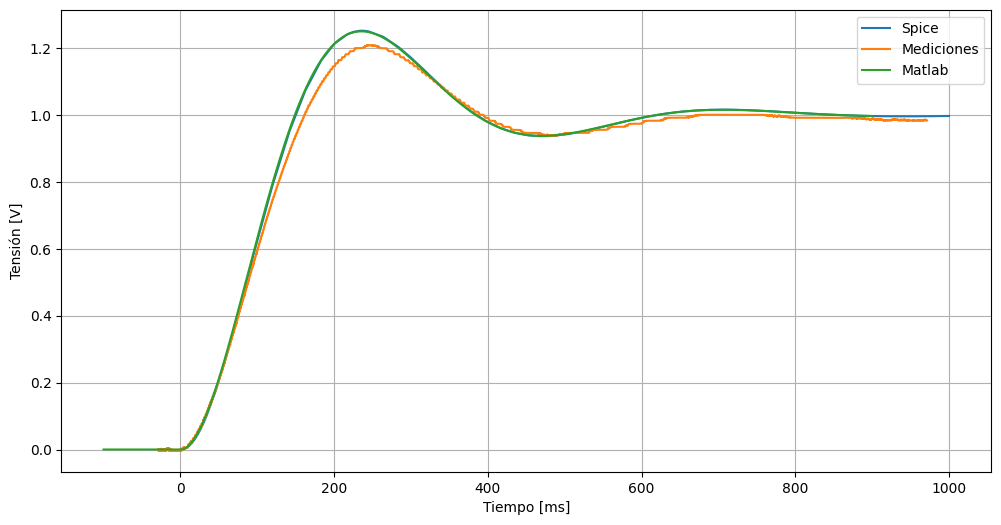
\includegraphics[width=0.8\textwidth]{Imagenes/4_Comparacion-Resultados/1_Lazo-Cerrado.png} % Reemplazar con el nombre de tu archivo
	\caption{Respuesta al escalón del sistema a lazo cerrado completo.}
	\label{fig:step_full}
\end{figure}

Las leves diferencias en el sobrepico y el estado estacionario pueden atribuirse a las tolerancias de los componentes pasivos y a las no linealidades propias de los amplificadores operacionales que no se contemplan en el modelo ideal.
\newpage
\subsection{Análisis en el Plano de Fase}
Para complementar el análisis temporal, se trazó el plano de fase (Derivada de la Salida vs. Salida) para ambos escenarios. 

En el sistema completo (Figura \ref{fig:fase_full}), la trayectoria describe una espiral convergente que se estabiliza rápidamente en el punto de equilibrio. La medición física se inscribe ligeramente por dentro de la curva de Matlab, lo que concuerda con el menor sobrepico observado en el dominio del tiempo.
\begin{figure}[H]
	\centering
	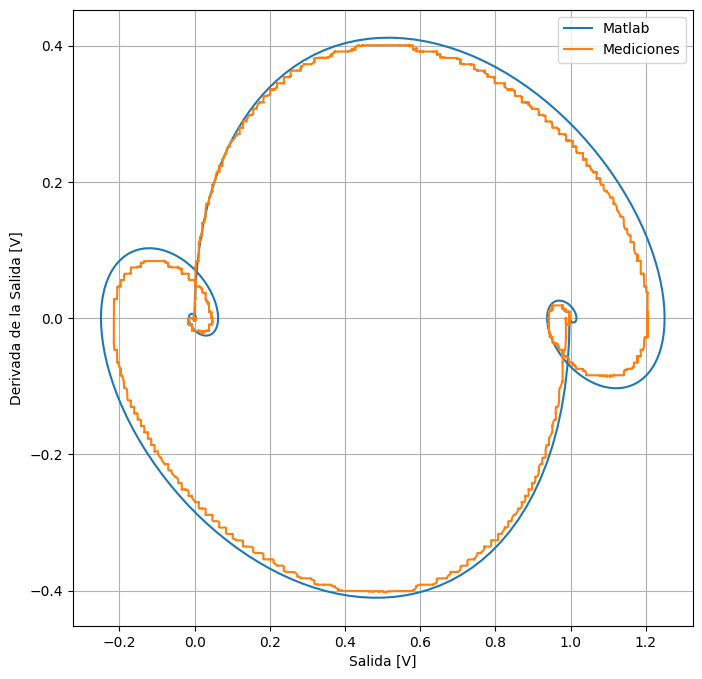
\includegraphics[width=0.6\textwidth]{Imagenes/4_Comparacion-Resultados/3_Fase-Completo.png} % Reemplazar con el nombre de tu archivo
	\caption{Plano de fase del sistema a lazo cerrado completo.}
	\label{fig:fase_full}
\end{figure}
